\documentclass{article}

\usepackage{graphicx}
\usepackage{tikz}
\usepackage{tikzsymbols}
\usetikzlibrary{calc,patterns,shapes.geometric}
\pagestyle{empty}
\usepackage[margin=0pt]{geometry}
\geometry{papersize={14in,12in}}

\def\centerarc[#1](#2)(#3:#4:#5){\draw[#1] ($(#2)+({#5*cos(#3)},{#5*sin(#3)})$) arc (#3:#4:#5);}

\begin{document}
	\begin{figure}
		\centering
		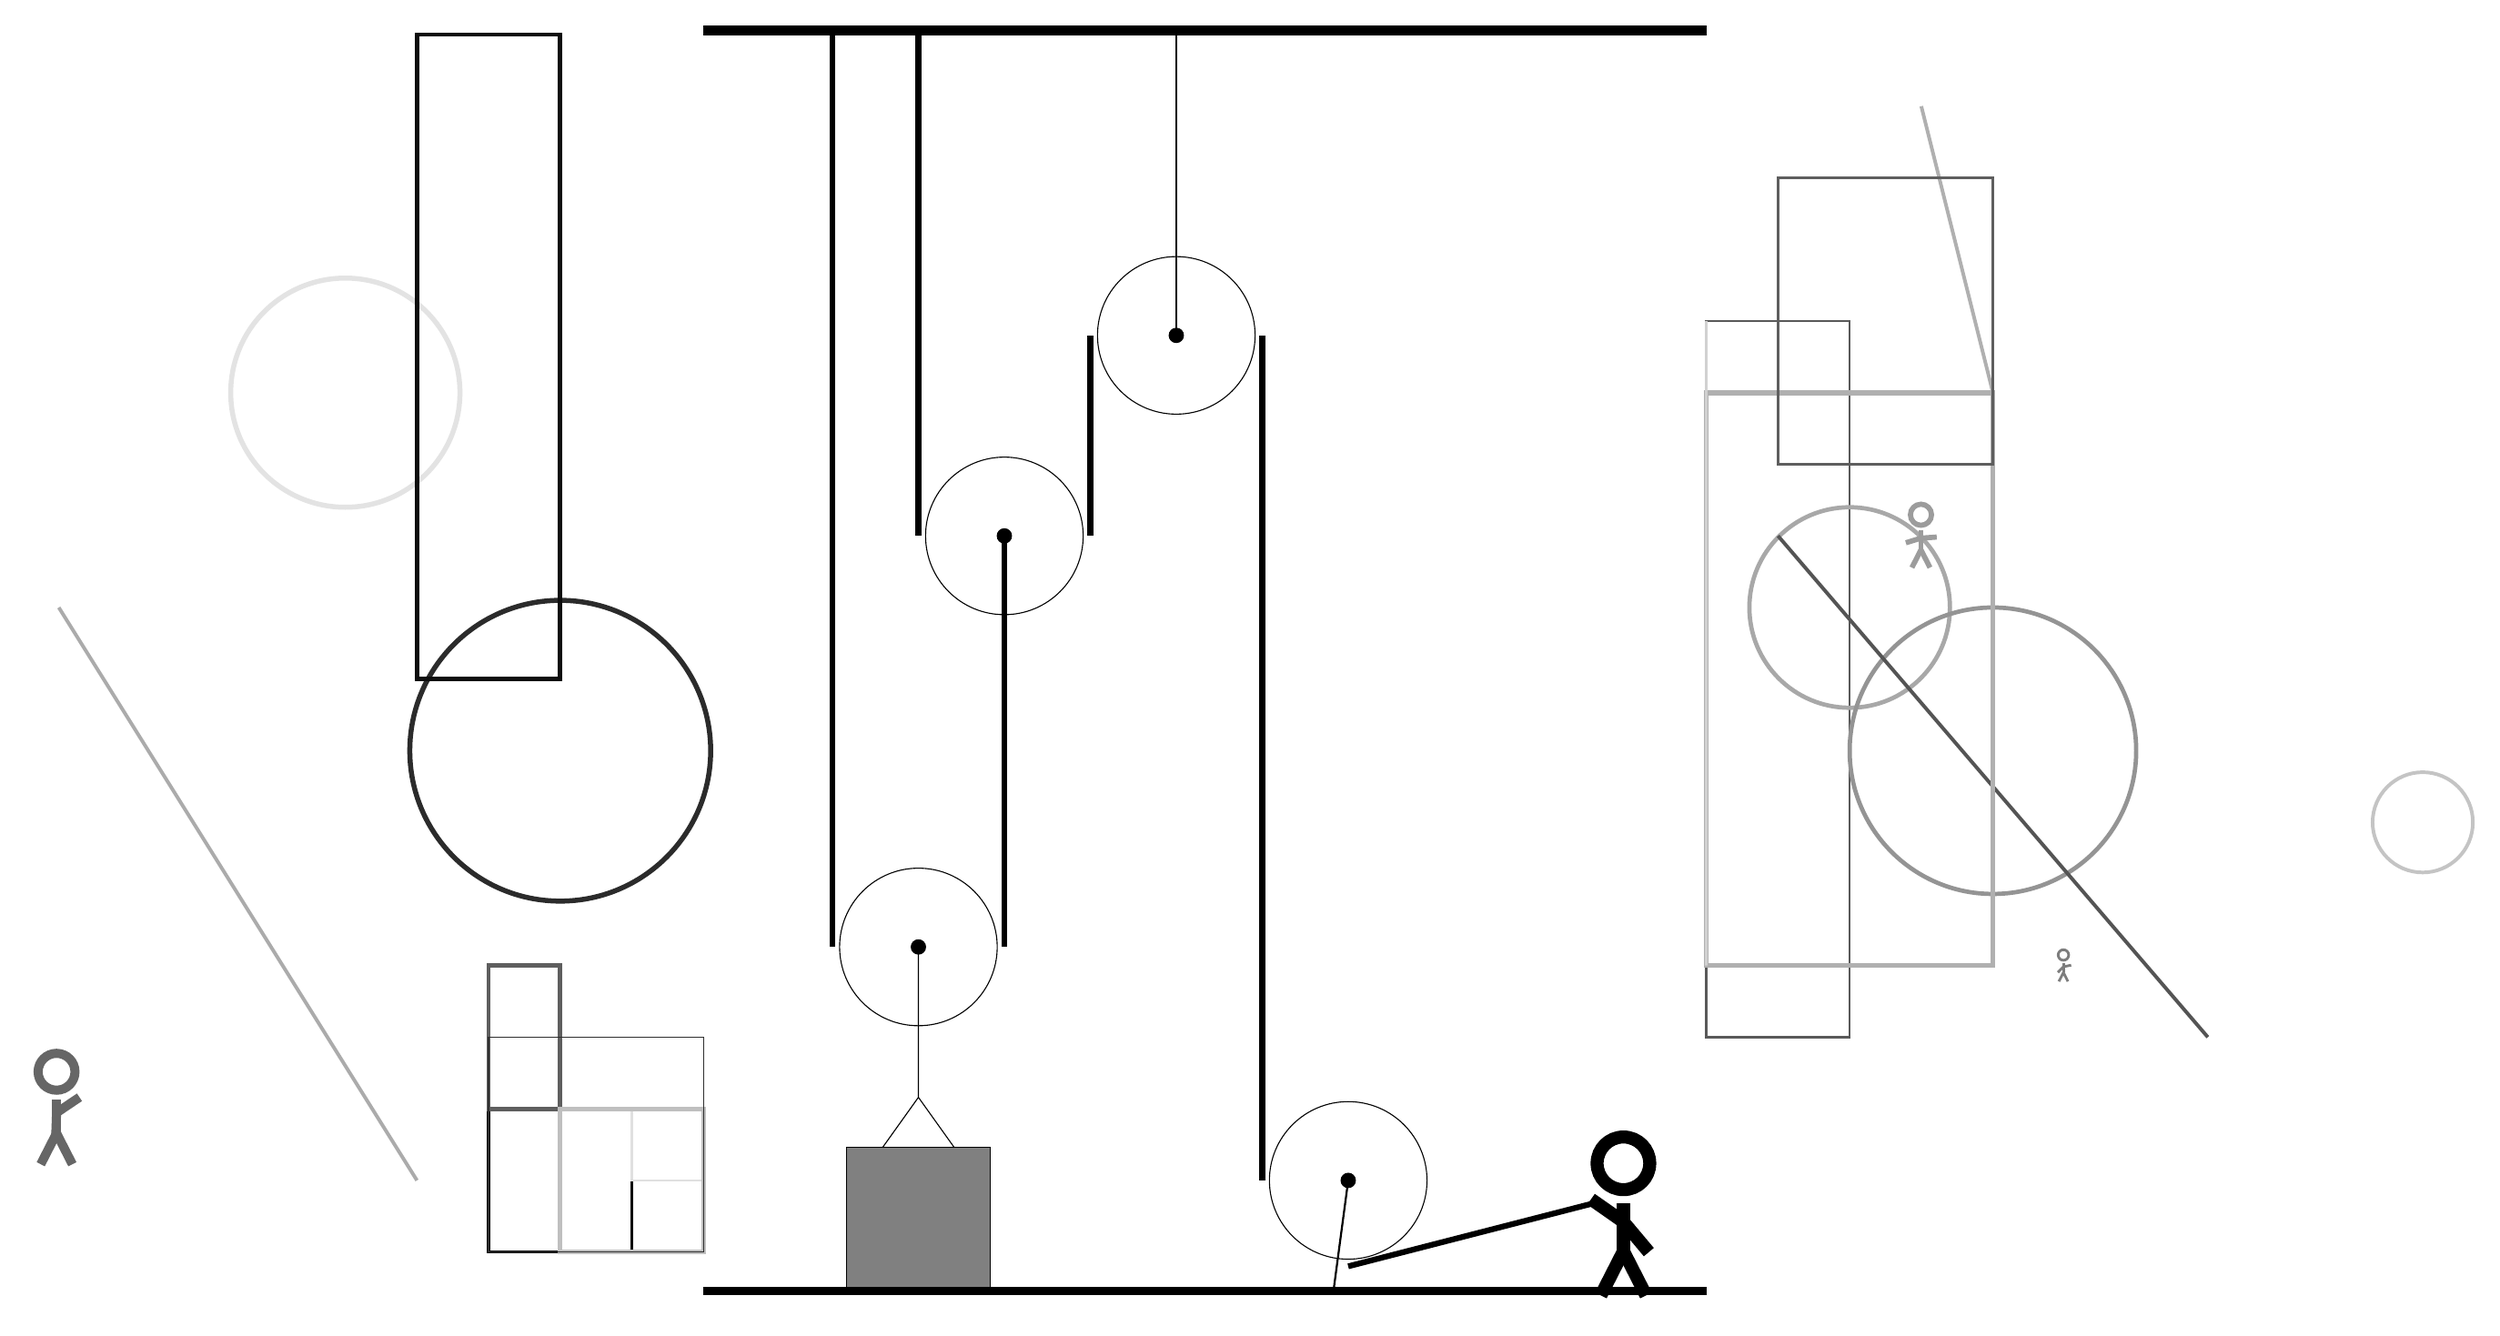
\begin{tikzpicture}
			%%%%% START %%%%%
			
			\draw[fill=black] (-2, 14) rectangle (12, 14.125);
			
			\draw (1, 1.26) circle (1.1);
			\draw[fill=black] (1, 1.26) circle (0.1);
			
			\draw [line width=0.3mm, color=black!38](-4, 8) circle (0.0);
			
			\node[line width=0.5mm, color=black!51] at (17, 1) {\Strichmaxerl[2][46][11]};
			\draw[line width=0.3mm, color=black!65] (12, 0) rectangle (14, 10);
			\draw [line width=0.6mm, color=black!34](14, 6) circle (1.4);
			\draw[line width=0.5mm, color=black!33](-6, -2) -- (-11, 6);
			\draw [line width=0.6mm, color=black!42](16, 4) circle (2.0);
			
			\draw[line width=0.5mm, color=black!31](15, 13) -- (16, 9);
			
			\draw [line width=0.5mm, color=black!90](-2, 4) circle (0.0);
			\draw[line width=0.4mm, color=black!96] (-3, -1) rectangle (-5, -3);
			\draw[line width=0.5mm, color=black!67](13, 7) -- (19, 0);
			\draw[line width=0.6mm, color=black!63] (-4, -1) rectangle (-5, 1);
			
			\draw[line width=0.7mm, color=black!31] (12, 9) rectangle (16, 1);
			\draw[line width=0.3mm, color=black!12] (-3, -1) rectangle (-2, -2);
			\draw [line width=0.5mm, color=black!23](22, 3) circle (0.7);
			\draw[line width=0.6mm, color=black!25] (-2, -3) rectangle (-4, -1);
			\draw [line width=0.7mm, color=black!11](-7, 9) circle (1.6);
			
			\node[line width=0.3mm, color=black!39] at (15, 7) {\Strichmaxerl[4][17][4]};
			\draw [line width=0.7mm, color=black!83](-4, 4) circle (2.1);
			\draw[line width=0.4mm, color=black!18] (12, 10) rectangle (12, 1);
			\draw[line width=0.3mm, color=black!63] (13, 12) rectangle (16, 8);
			\draw[line width=0.6mm, color=black!95] (-4, 14) rectangle (-6, 5);
			\node[line width=0.3mm, color=black!60] at (-11, -1) {\Strichmaxerl[7][88][34]};
			\draw[line width=0.2mm, color=black!82] (-2, 0) rectangle (-5, -3);
			
			\draw (2.2, 7.0) circle (1.1);
			\draw[fill=black] (2.2, 7.0) circle (0.1);
			
			\draw (4.6, 9.8) circle (1.1);
			\draw[fill=black] (4.6, 9.8) circle (0.1);
			\draw[thick] (4.6, 9.8) -- (4.6, 14);
			
			\draw (7.0, -2) circle (1.1);
			\draw[fill=black] (7.0, -2) circle (0.1);
			\draw[thick] (7.0, -2) -- (6.8, -3.5);
			
			\draw (1, 1.26) -- (1, -0.84) -- (0.5, -1.54) -- (1.5, -1.54) -- (1, -0.84);
			\draw[fill=black!50] (0, -1.54) rectangle (2, -3.54);
			\draw[line width=0.8mm] (-0.2, 14) -- (-0.2, 1.26);
			\centerarc[line width=0.8mm](1, 1.26)(180:360:1.2000000000000002);
			\draw[line width=0.8mm](2.2, 1.26) -- (2.2, 7.0);
			\draw[line width=0.8mm] (1.0, 14) -- (1.0, 7.0);
			\centerarc[line width=0.8mm](2.2, 7.0)(180:360:1.2000000000000002);
			\draw[line width=0.8mm](3.4, 7.0) -- (3.4, 9.8);
			\centerarc[line width=0.8mm](4.6, 9.8)(0:180:1.2000000000000002);
			\draw[line width=0.8mm] (5.8, 9.8) -- (5.8, -2);
			\centerarc[line width=0.8mm](7.0, -2)(0:90:-1.2000000000000002);
			\draw[line width=0.8mm](7.0, -3.2) -- (10.5, -2.3);
			
			\node at (10.8, -2.5) {\Strichmaxerl[10][-35][-50]};
			
			\draw[fill=black] (-2, -3.5) rectangle (12, -3.6);
			
			%%%%% END %%%%%
		\end{tikzpicture}
	\end{figure}	
\end{document}